\section{Spread Simulation and Prediction}
In this section, we build pest's population migration model based on its special population characteristics and predict its distribution over time. We utilize the \textbf{Cellular Automata (CA)} to simulate the spread of pest and establish transition rule based on population migration characteristics. We name our model as \textbf{Pest Spread-Cellular Automata(PS-CA)} model. Finally we get the distribution map of pests spread over time, analyze the spread situation and study the precision of our model.%等到扩充

%%第一部分 建模
\subsection{Spread Simulation Preparations based on Cellular Automata}
Cellular Automata (CA) is an array of finite automata connected locally, which update their states in discrete time and at the same moments; every automaton updates its next state depending on the states of its closest neighbors \parencite{CA}. For example, Huynh, HX and his collegues have studied the spread of brown plant hoppers based on cellular automata \parencite{CAtheorem}. Similarly in this problem, we are going to predict the population migration of vespa mandarinia on the basis of cellular automata.

In the manner of formal language, cellular automata can be discribed as a 4-tuples:

\begin{equation*}
    \text{CA} = (L^d, S, N, f)
\end{equation*}
where CA is the cellular automata system, $L$ represents a regularly divided grid space, and each grid space is a cell, $d$ is the dimension of $L$, $S$ is a discrete finite set, $N$ symbolizes the neighbour set of cellular and $f$ is the transition rule.

To be specific, for each $N \subset L$, let the number of cells in the neighbor set be denoted as $n$, then $N$ can be interpreted as a combination of cells in a domain, that is, a space vector containing $n$ different cell states. Recorded as:

\begin{equation*}
    N = (s_1, s_2, \dots, s_n), s_i \in L, i \in (1, \dots, n)
\end{equation*}

Meanwhile, $f$ implies a mapping function: $S^n_t \xrightarrow{} S_{t+1}$. In other words, the state value of the cell at $t+1$ moment is determined by all the neighbours' state at $t$ moment. We will analyze it in detail in the next part.

After understanding the theorem of CA, we need to contruct a cellular automata model that fits the spread of pest, and the most important part is transition rule. In the beginning, let us make some bold assumptions:

\begin{itemize}
    \item \textbf{Natural enemies of pest are ignored.} Since the natural enemies of Vespa mandarinia have little effect on its containment and the types of natural enemies are too complex, we ignore this factor.
    \item \textbf{Its growth curve conforms to the J-curve.} When the foreign organisms invade, their survival pressure is at a low level, so the initial growth will be J-shaped. Our problem situation is exactly when the pests broke out rapidly in the early stage, so we can assume that its growth mode is J-type, except for its hibernation.%最好找到参考文献
    \item \textbf{The hibernation period of pests is from January to April.} When we observe the time of sighting of positve events, we find that they all occur from May to December, and this assumption is consistent with the pest’s living habits due to temperature changes.
\end{itemize}

On the basis of the former assumptions, our model construction and variable definition are accomplished through the following steps:

\begin{enumerate}[\quad\bf Step1.]
%%1
\item
We define the simulation area of Washington State. In order to include as more positive reports as possible, we define the simulation area from $123.9254^{\circ} W$ to $120.7114^{\circ} W$ in longitude and from $47.7294^{\circ} N$ to $49.1550^{\circ} N$ in latitude. The selected area is shown in Figure \ref{fig:2021C-The selected simulation area.} and it is also used in step 6 for our initialization.

In our model, we simply regard our simulation area as a rectangle and divide it into a lot of small ones, which represent a cell in our cellular automata model.

% The selected area is shown in Figure \ref{fig:2021C-The selected simulation area.}, and it is also used in step 6 to classify the geographical environment value, which is shown in Figure \ref{fig:2021C-Classification of geographical environment value.}.

%%2
\item
We denote a few notations in Table \ref{tbl:2021C-Notations of cellular automata}, including all the variable we use in our model.
%%三线表 cellular automata notation
\begin{table}[H]
    \renewcommand\arraystretch{2}   %%控制行间距
    \centering
    \caption{Notations of cellular automata.}
    \begin{tabular}{ccc}    %%三列均左对齐
        \toprule  %%表格横线加粗
        \specialrule{0em}{2pt}{2pt}    %%添加透明线控制行高
        Symbol & Definition & Notes \\
        \specialrule{0em}{2pt}{2pt}    %%添加透明线控制行高
        \midrule
        \specialrule{0em}{1pt}{1pt}
        $A$ & the set of n areas in the simulation area & $A = \{ a_1, a_2, \dots, a_n \}$ \\
        $X$ & the set of horizontal coordinates & $X = \{ x_1, x_2, \dots, x_n \}$ \\
        $Y$ & the set of vertical coordinates & $Y = \{ y_1, y_2, \dots, y_n \}$ \\
        $GE$ & the set of geographical environment & $GE = \{ ge_1, ge_2, \dots, ge_n \}$ \\
        $P$ & the set of pest with an ideal population growth & $P = \{ p_{1,t}, p_{2,t}, \dots, p_{n,t} \}$ \\
        $M$ & the set of migration & $M= \{ m_{1,t}, m_{2,t}, \dots, m_{n,t} \}$ \\
        $V^c$ & the set of current volume of pest & $V^c = \{ v^c_{1,t}, v^c_{2,t}, \dots v^c_{n,t}$ \} \\
        $S$ & the state of the cell & $S = \{ s_{1,t}, s_{2,t}, \dots, s_{n,t}$ \}\\
        $d_{max,t}$ & The maximum distance of spread at time t &  \\
        % $c^s_t$ & the spread coefficient at time $t$  & \\
        
        \specialrule{0em}{1pt}{1pt}
        \bottomrule
    \end{tabular}
    \label{tbl:2021C-Notations of cellular automata}
\end{table}

Each cell represents an area, which is described by coordinate $x$ and $y$. Moreover, we also take other factors into consideration, such as the geographical environment $ge$, the population growth of pests $p_{i,t}$ and the current volume $v^e_{i,t}$. Now we get the cellular automata model as follows:

\begin{equation*}
    A = L^6 = (X \times Y \times GE \times P \times M\times V^c),
\end{equation*}
% where $A_i$ at the time $t$ is presented by $(x_i,y_i,ge_i,m_i,v^c_{1,t})$
where $a_i$ at the time $t$ is presented by $(x_i, y_i, ge_i, p_{i,t},m_{i,t},v^c_{i,t})^T$.


%%3
\item
We clarify the meaning of the cell state. Each cell is assigned a state at a time and it describes the degree of the pest gathering, which can imply the likelihood that the citizen in this area report to discover Asian giant hornets. At a specific time $t$, we simply let the current volume $v^c_{i,t}$ be the state of an area $s_{i,t}$, so that $s_{i,t} = v^c_{i,t}$ can be displayed directly the possibility of pest occurrence.

%%4
\item
We determine the neighborhood vector by using the Moore neighborhood method. Through this method, the central cell is related to its eight surrounding cells like Figure \ref{fig:2021C-The Moore neighborhood method.}.

%%图片 Moore neighborhood method
\begin{figure}[H]
    \centering
    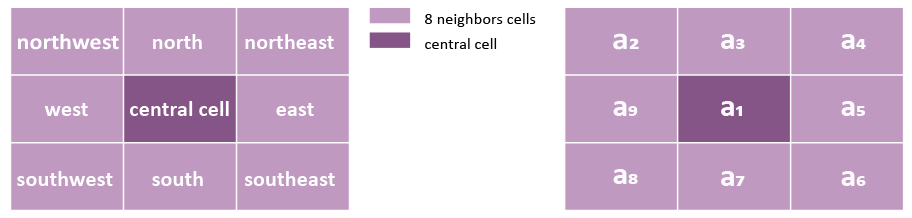
\includegraphics[scale = 0.4]{Chapter-2021C/images-2021C/1-mooer.png}
    \caption{The Moore neighborhood method.}
    \label{fig:2021C-The Moore neighborhood method.}
\end{figure}

For the central cell, its neighbors are presented by a set N with $$N = \{a_2, a_3, a_4, a_5, a_6, a_7, a_8, a_9\}$$ Next, we will use this subscript variable to do a small calculation description.

%%5
\item
Next, We consider the transition rule of the current volume $v^c_{i,t}$.

According to the living habits of the pests that they actively appears in months from May to December when the queen start to build new nest and reproduce. Therefore, we stop simulation from January to April and restart it at the beginning of May.

As for the $i^{th}$ area, the current volume at $t+1$ moment $v^c_{i,t+1}$ depends on the number of pest population growth at $t$ moment $p_{i,t}$ and the number of migration at $t+1$ moment.
For clarity, we only calculate and explain within the range of Moore  neighborhood, that is, $i= 1,2,\dots,9$.
According to the J-curve, we know that 
    $$p_{i,t} = N_0 \times \lambda^t$$ 
where $N_0$ and $\lambda$ are constant, and
    $$\frac{p_{i,t+1}}{p_{i,t}} = \frac{N_0 \times \lambda^{t+1}}{N_0 \times \lambda^t} = \lambda$$ 
Then we have  $$p_{i,t+1} = \lambda \times p_{i,t}$$
We define the number of pest migration in central cell as depending on its current volume and the geographical environment of its eight neighbors.
    \begin{equation*}
        \label{equ:transition rule}
        m_{1,t} = \frac{ge_k}{ge_k+4} \times v^c_{1,t}, 
    \end{equation*}
where $ge_k = max \{ ge_i \} (i=2, 3, \dots, 9)$ is the maximum of the $ge$ of the neighbor cells.
In all, we achieve the transition rule that is 
    $$v^c_{1,t+1} = \lambda \times p_{1,t} + m_{1,t}.$$
\vspace{-0.6cm}
%%6
\item
We initialize the value of the geographical environment set $GE$ as Figure \ref{fig:2021C-Process of GE.} shows and the starting point. Then we search and get the simulation area map according to Figure \ref{fig:2021C-The selected simulation area.} and the legend in it\parencite{GoogleMap}. The figure shows the vegetation coverage of this area.

The pest typically build their nests underground, usually in abandoned
rodent burrows in forests\parencite{attachment}. So we infer that pest is more likely to migrate to places with lush vegetation. We classify the value of $ge_i$ for each cell according to the difference of vegetation coverage in Figure \ref{fig:2021C-Classification of GE.}. In detail, we allocate rivers and regions with no vegetation coverage with value 0. Additionally, we grant the value of 4, 3, and 1 to the areas with the green colour from deep to shallow. The result can be seen in Figure \ref{fig:2021C-Value Allocation of GE.}. In conclusion, the bigger the value of $ge_i$ is, the more likely it is for the pests to migrate to this area.

% \begin{figure}[H] 
% \begin{minipage}[t]{0.5\linewidth} 
% \centering 
% 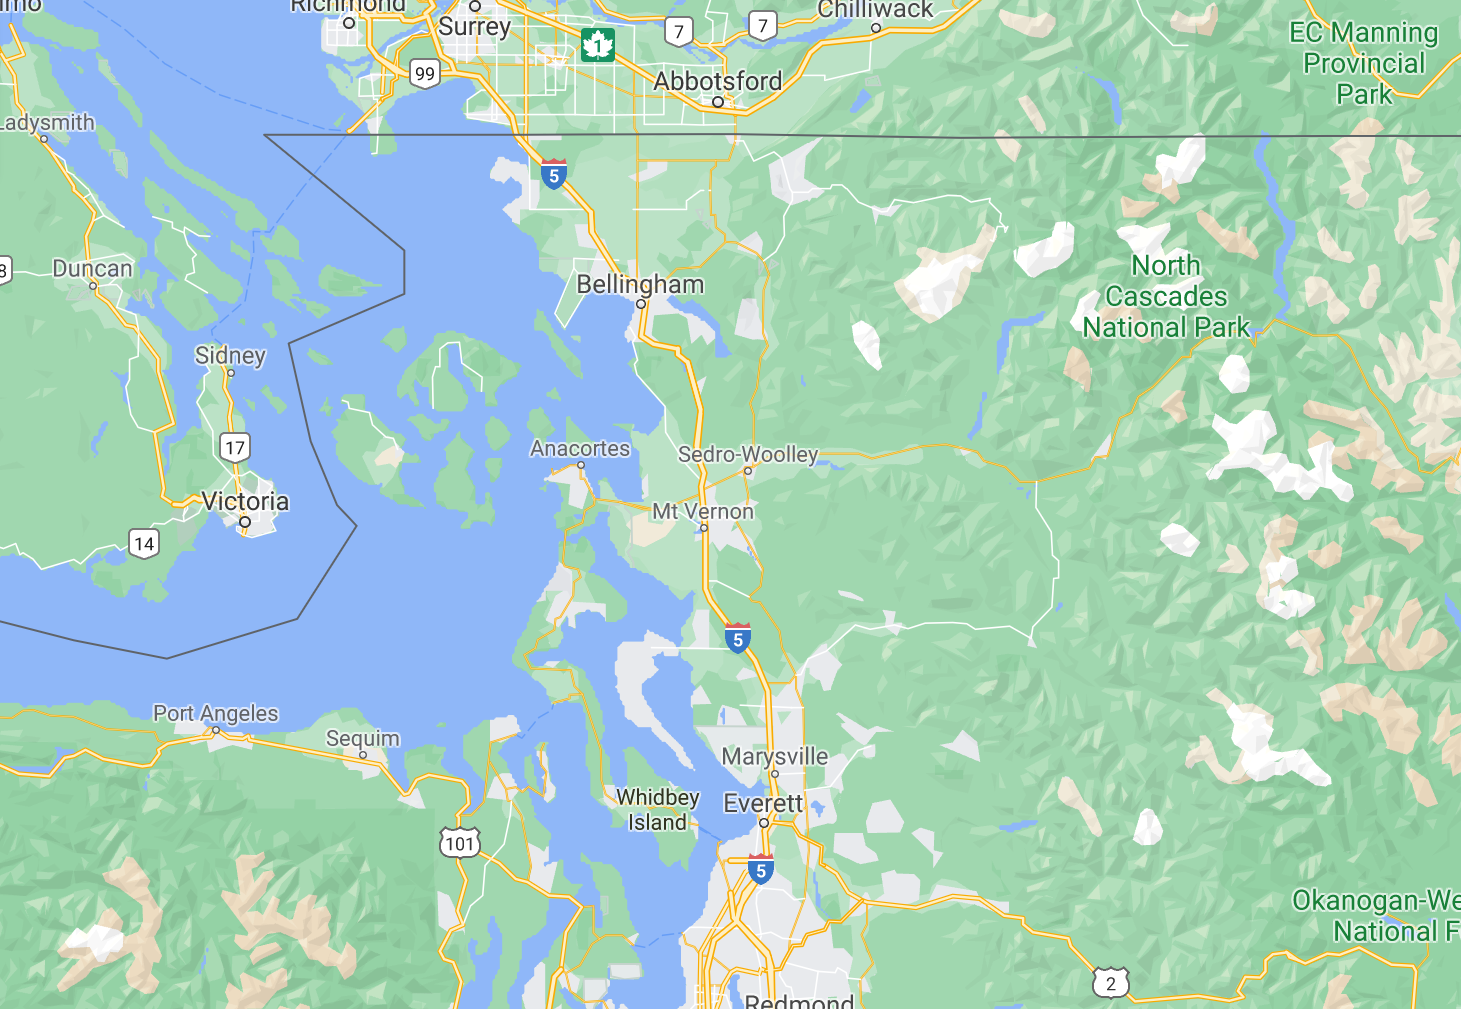
\includegraphics[width=2.5in]{Chapter-2021C/images-2021C/1-map.png} 
% \caption{The selected simulation area.} 
% \label{fig:2021C-The selected simulation area.} 
% \end{minipage}
% \begin{minipage}[t]{0.5\linewidth} 
% \centering 
% 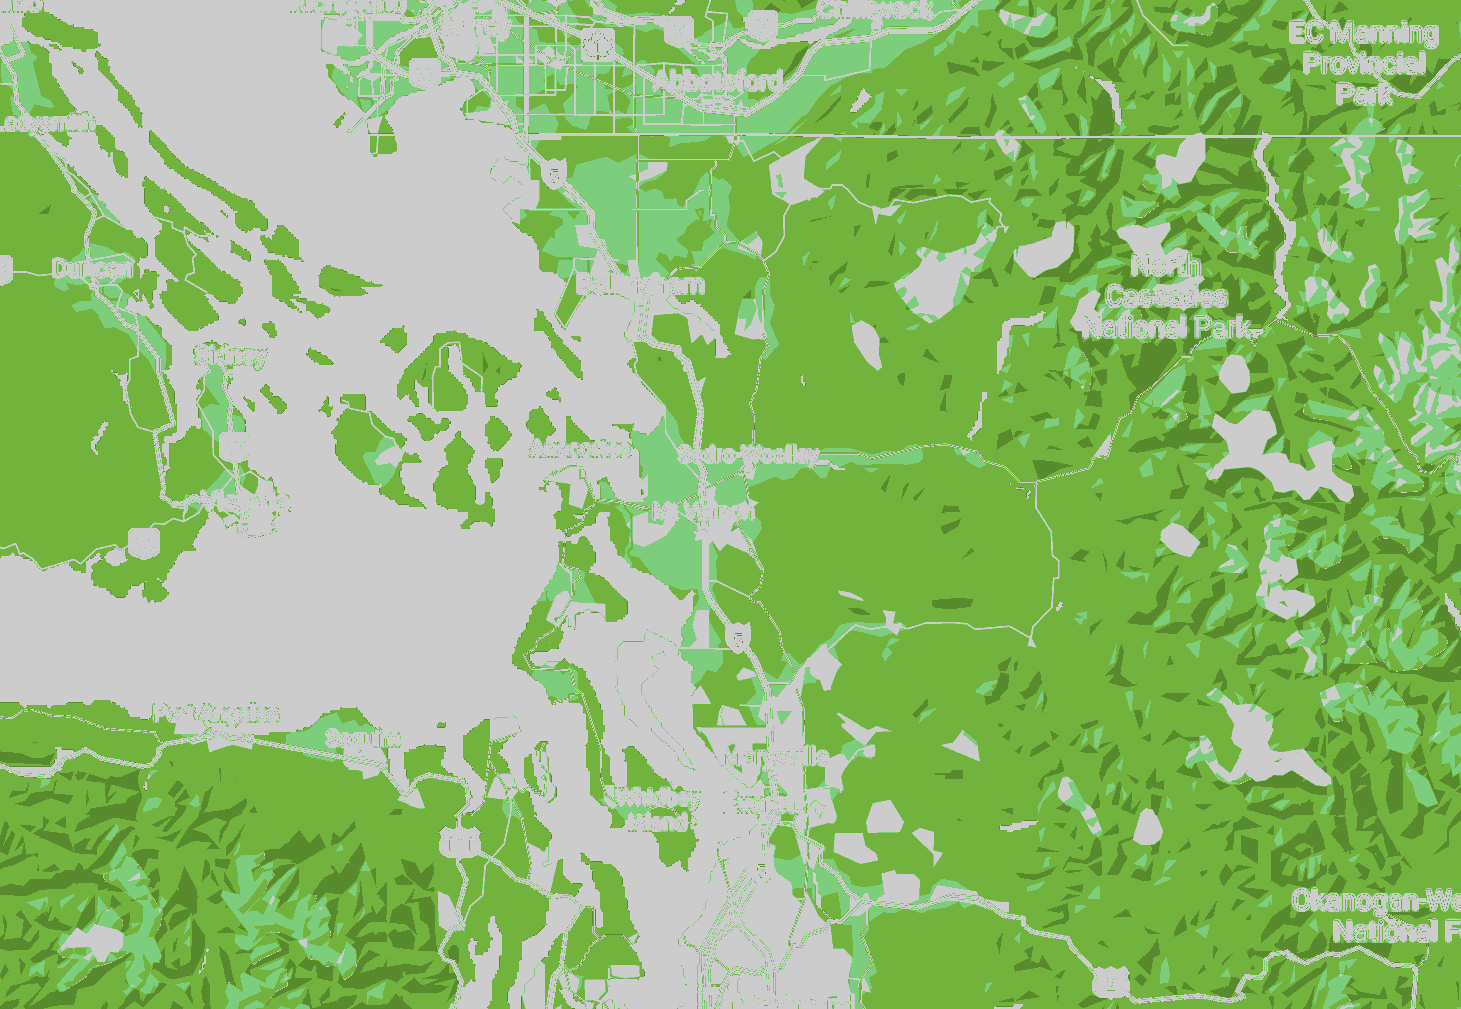
\includegraphics[width=2.5in]{Chapter-2021C/images-2021C/1-classification.png} 
% \caption{Classification of $GE$.} 
% \label{fig:2021C-Classification of GE.} 
% \end{minipage} 
% \end{figure}

\begin{figure}[H]
\centering
\subfigure[Simulation area.]{
\begin{minipage}[t]{0.33\linewidth}
\centering
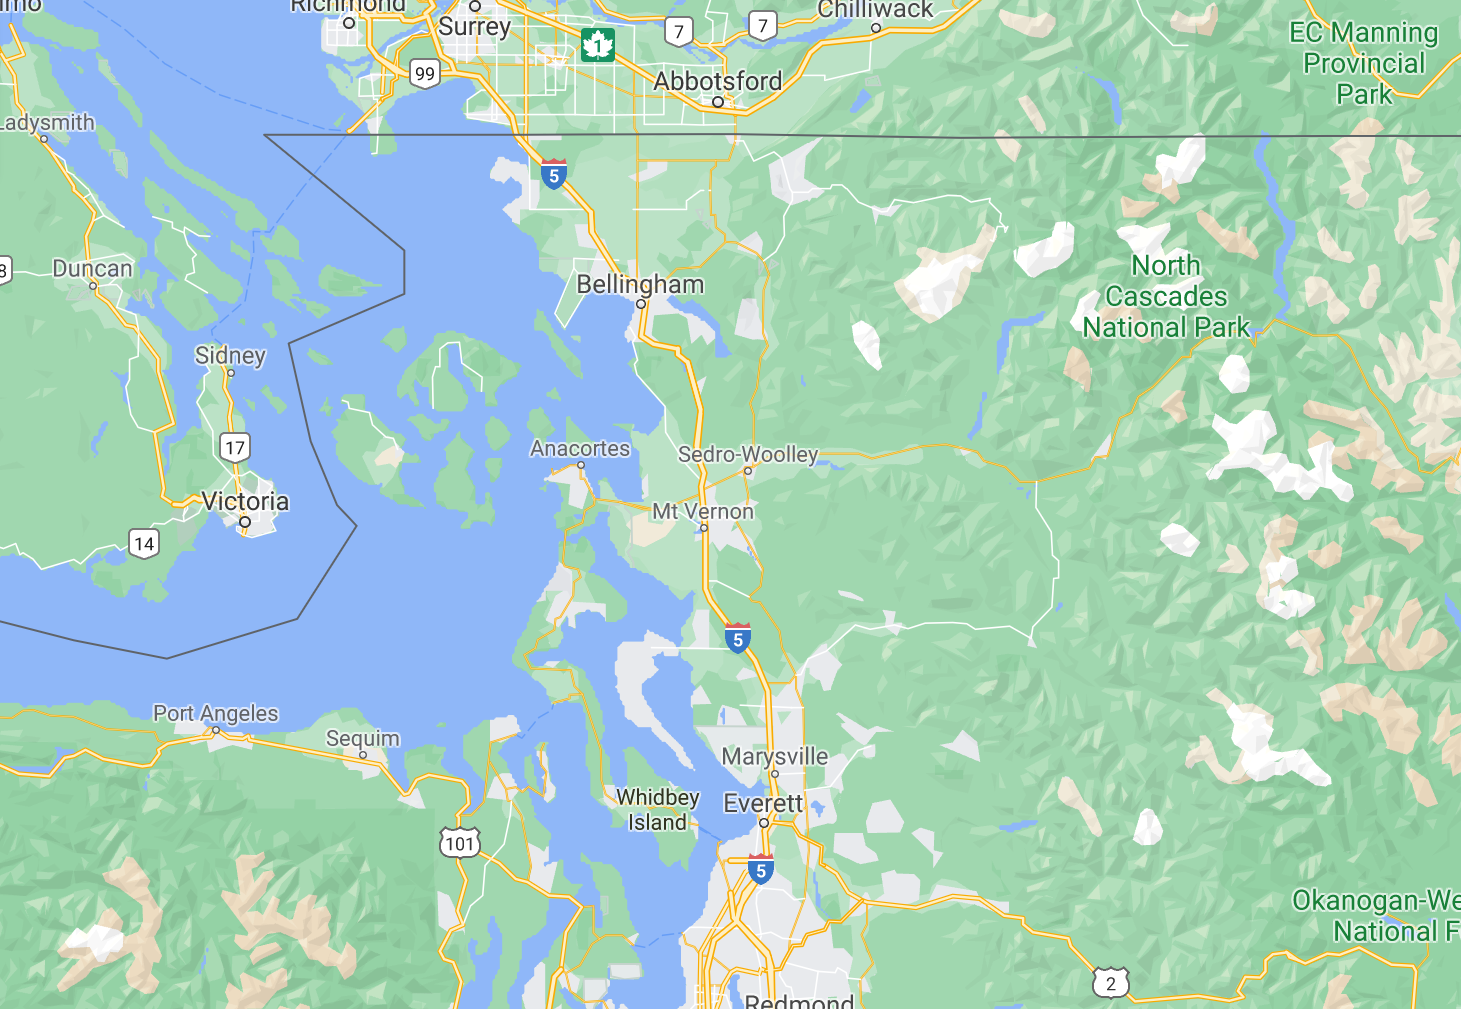
\includegraphics[width=1.7in]{Chapter-2021C/images-2021C/1-map.png}
%\caption{fig1}
\label{fig:2021C-The selected simulation area.} 
\end{minipage}%
}%
\subfigure[Classification of $GE$.]{
\begin{minipage}[t]{0.33\linewidth}
\centering
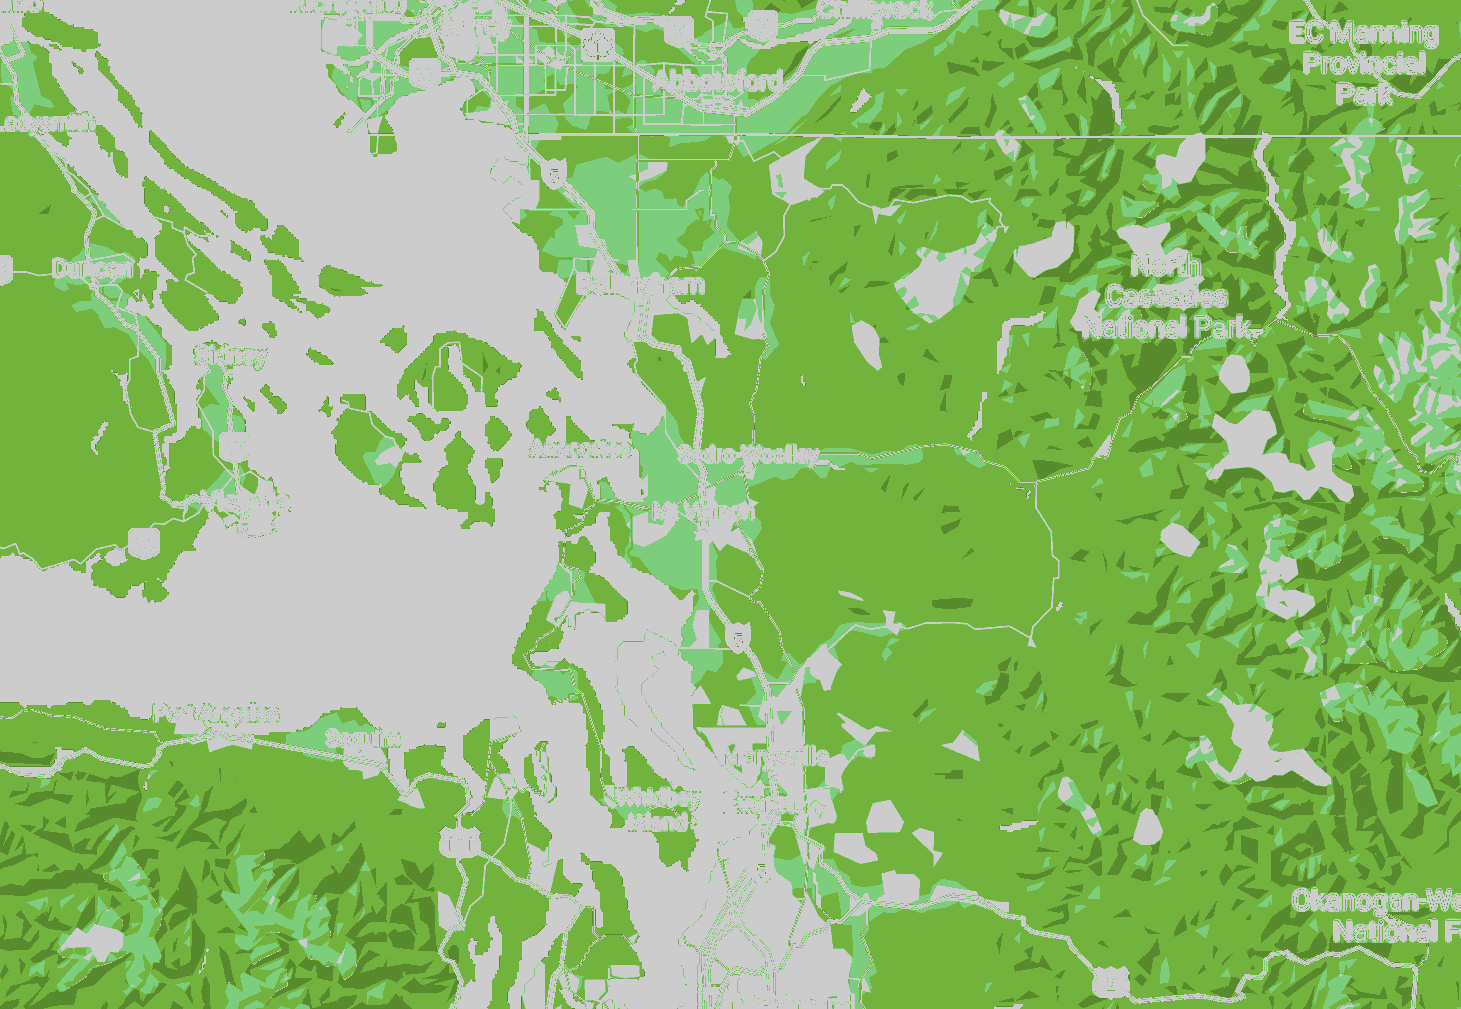
\includegraphics[width=1.7in]{Chapter-2021C/images-2021C/1-classification.png}
%\caption{fig2}
\label{fig:2021C-Classification of GE.} 
\end{minipage}%
}%
\subfigure[Value Allocation of GE.]{
\begin{minipage}[t]{0.33\linewidth}
\centering
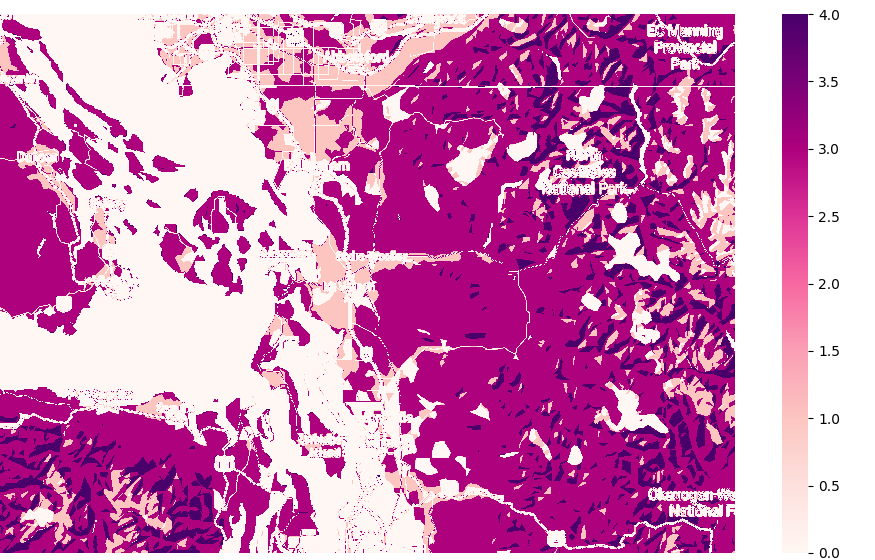
\includegraphics[width=1.9in]{Chapter-2021C/images-2021C/1-gescore.png}
%\caption{fig2}
\label{fig:2021C-Value Allocation of GE.} 
\end{minipage}
}%
\centering
\caption{Process of $GE$.}
\label{fig:2021C-Process of GE.} 
\end{figure}

\vspace{-0.5cm}

After that, we are ready to initialize the starting point and set the initial pest population $P_{i,1}$ and the value of constant $\lambda$. According to the detection time, the earliest positive report is at $(123.9431^{\circ}W , 49.149396^{\circ}N)$. However, the report place is far away from other ones and is blocked by a river. Additionally, no new positive reports emerge near it so that we ignore this report. Then we select the next report place $(122.7022^{\circ}W, 48.99389^{\circ}N)$ as the starting point on 2019/9/30. Moreover, we set the initial pest population $p_{start,1}$ as 200, the simulation time as 380 to include the detection time of the last positive report, and the constant $\lambda$ as $1.2$.

\end{enumerate}

\subsection{Spread Simulation Consequence}
After the above steps of preparation and initialization, we run the cellular automata. Then we get the simulation consequence of one year as Figure \ref{fig:2021C-Simulation of pest spread in one year.} shows and the one of two years as Figure \ref{fig:2021C-Simulation of pest spread in two years.} shows.

% \begin{figure}[H] 
% \begin{minipage}[t]{0.25\linewidth} 
% \centering 
% 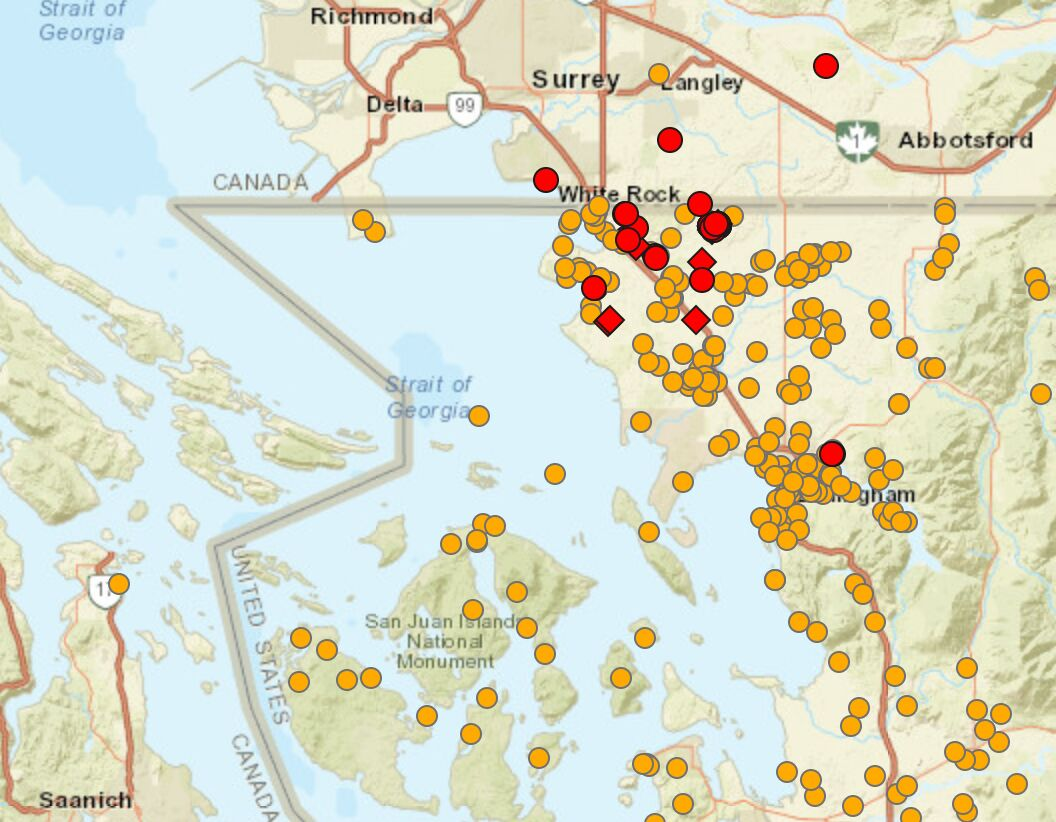
\includegraphics[width=1in]{Chapter-2021C/images-2021C/1-positive reality.jpg}
% \caption{Reality of positive reports.} 
% \label{fig:2021C-Reality of positive reports.} 
% \end{minipage}
% \begin{minipage}[t]{0.25\linewidth} 
% \centering 
% 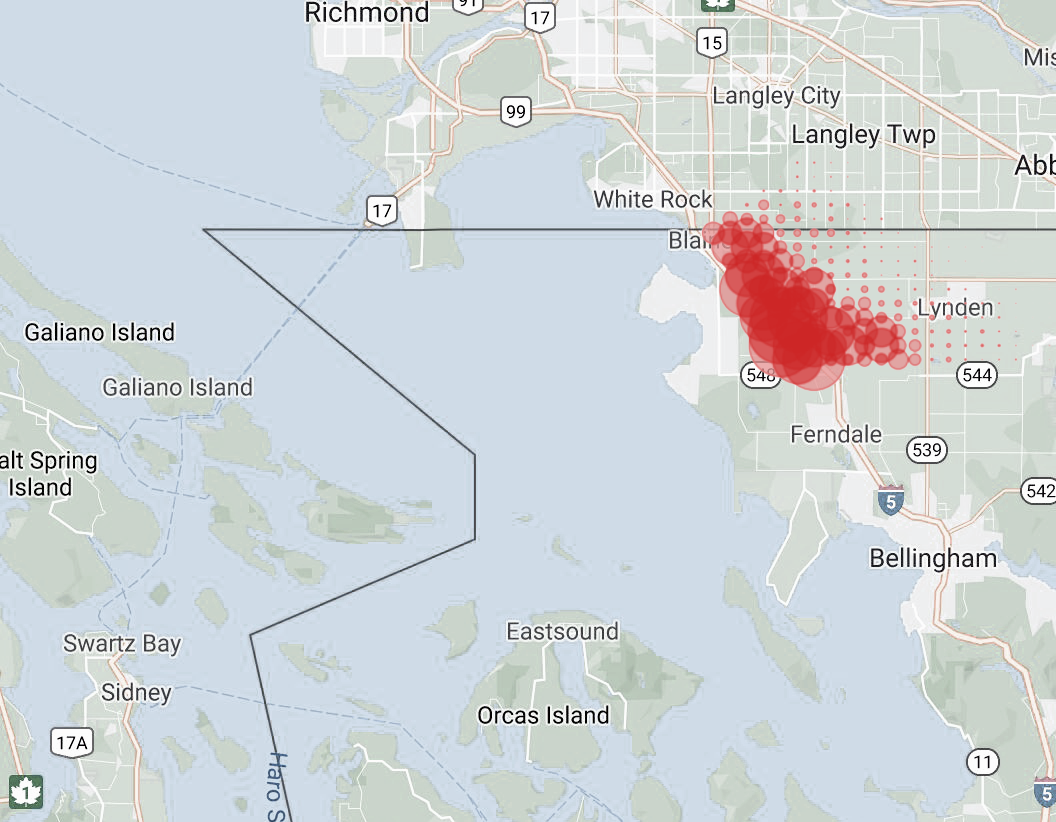
\includegraphics[width=1in]{Chapter-2021C/images-2021C/1-positive simulation.png} 
% \caption{Simulation of pest spread in one year.} 
% \label{fig:2021C-Simulation of pest spread in one year.} 
% \end{minipage} 
% \begin{minipage}[t]{0.25\linewidth} 
% \centering 
% 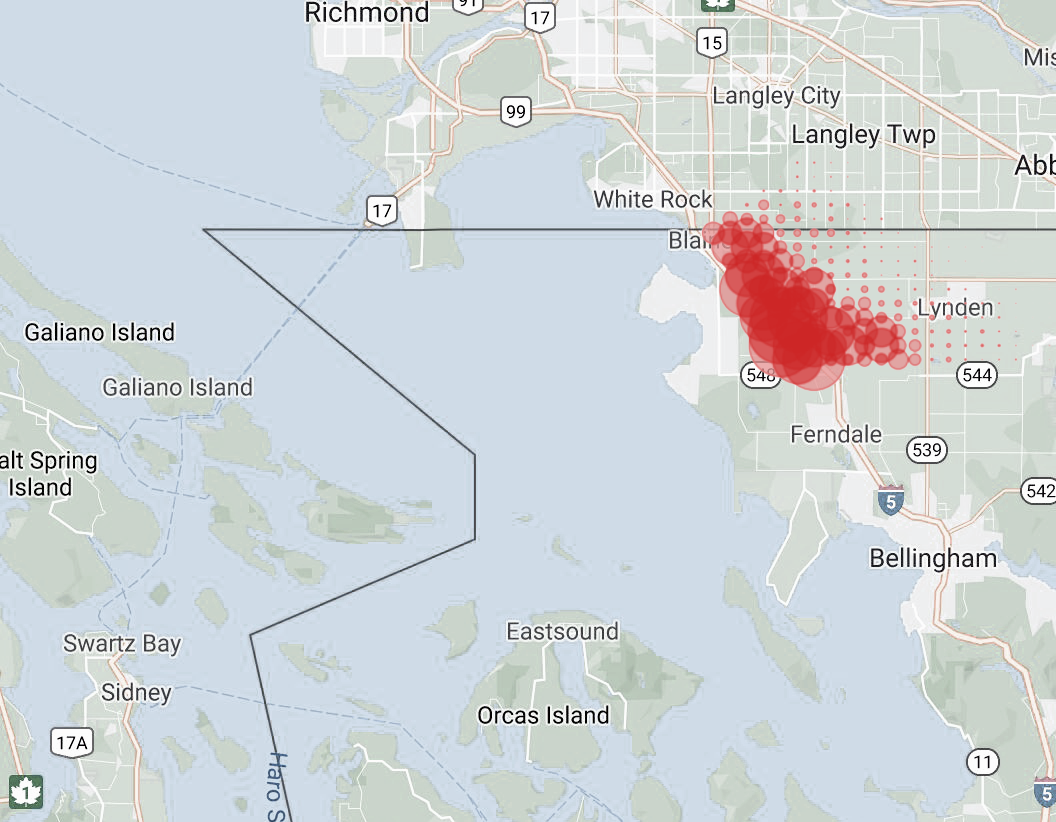
\includegraphics[width=1in]{Chapter-2021C/images-2021C/1-positive simulation.png} 
% \caption{Simulation of pest spread in two years.} 
% \label{fig:2021C-Simulation of pest spread in two years.} 
% \end{minipage} 
% \end{figure}

\begin{figure}[H]
\centering
\subfigure[Reality of positive reports.]{
\begin{minipage}[t]{0.33\linewidth}
\centering
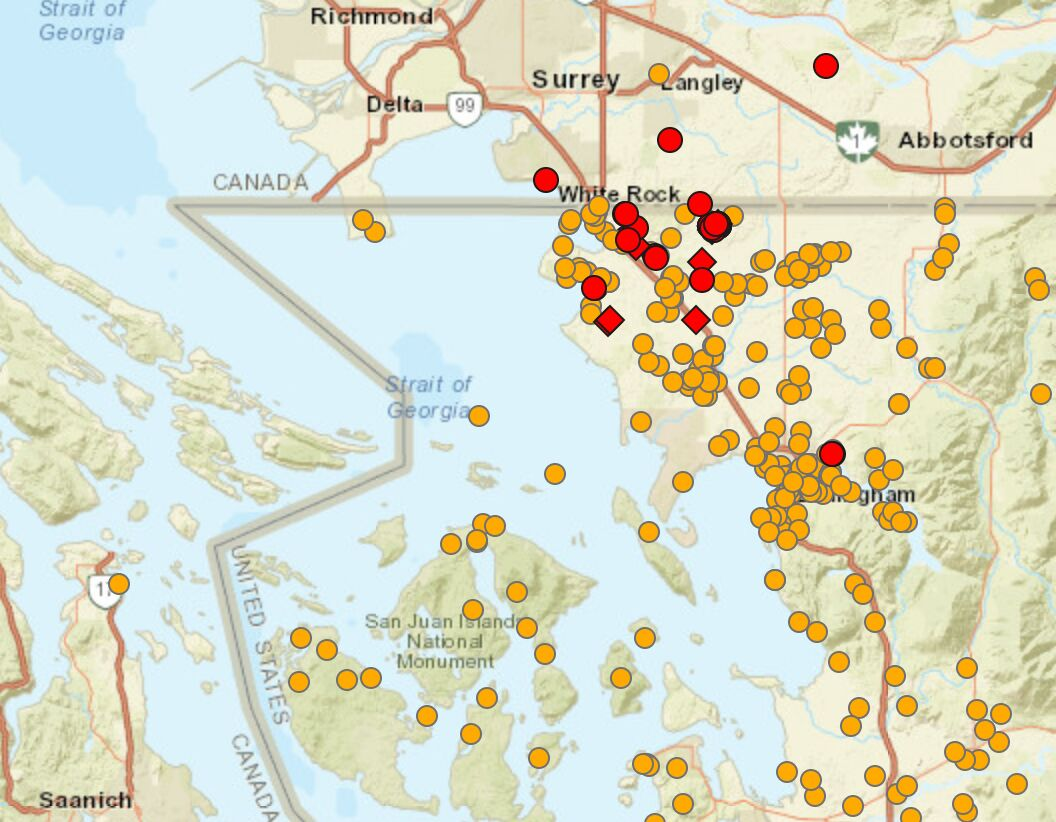
\includegraphics[width=1.7in]{Chapter-2021C/images-2021C/1-positive reality.jpg}
%\caption{fig1}
\label{fig:2021C-Reality of positive reports.} 
\end{minipage}%
}%
\subfigure[Simulation of one year.]{
\begin{minipage}[t]{0.33\linewidth}
\centering
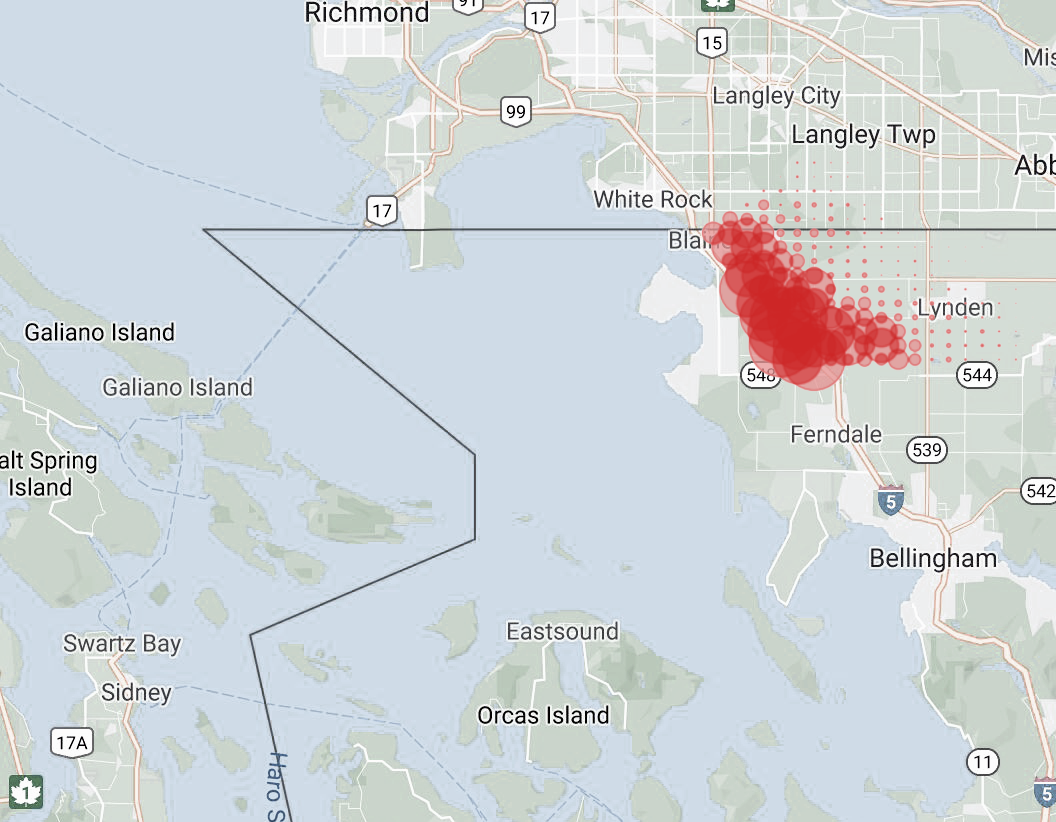
\includegraphics[width=1.7in]{Chapter-2021C/images-2021C/1-positive simulation.png}
%\caption{fig2}
\label{fig:2021C-Simulation of pest spread in one year.} 
\end{minipage}%
}%
\subfigure[Simulation of two years.]{
\begin{minipage}[t]{0.33\linewidth}
\centering
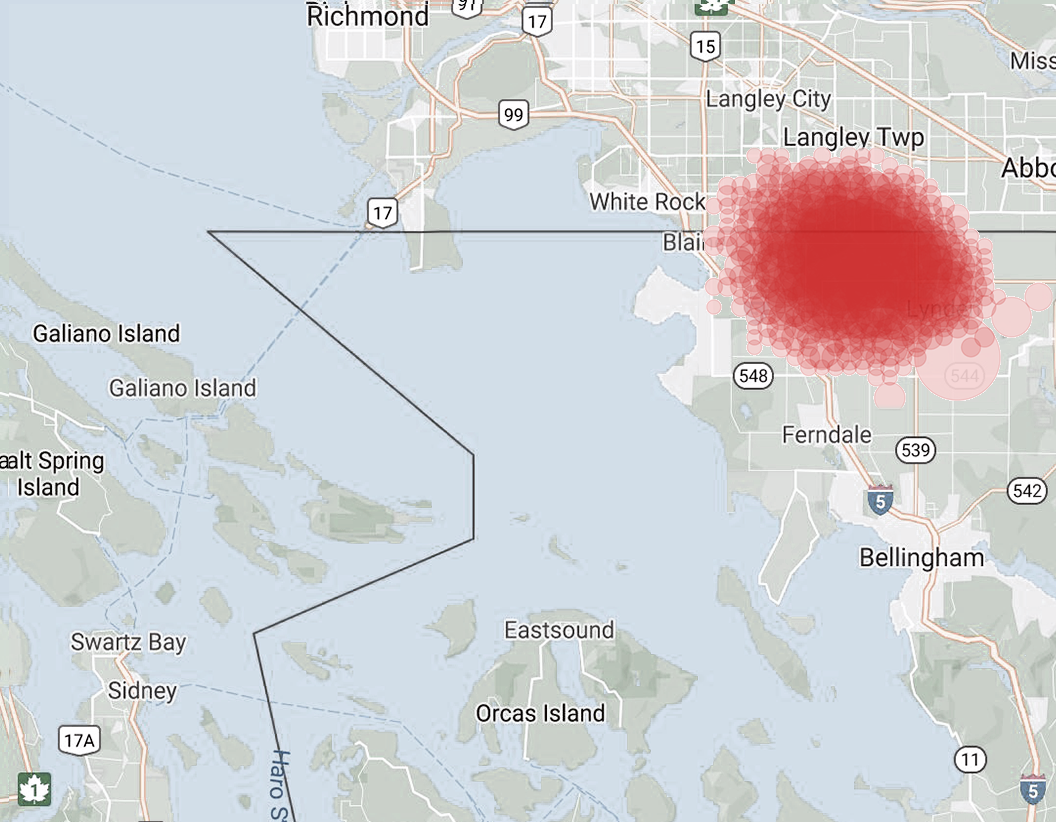
\includegraphics[width=1.7in]{Chapter-2021C/images-2021C/1-positive simulation2.png}
%\caption{fig2}
\label{fig:2021C-Simulation of pest spread in two years.} 
\end{minipage}
}%
\centering
\caption{Comparison of Reality and Simulation.}
\end{figure}

In Figure \ref{fig:2021C-Reality of positive reports.}, red points represent the real place of these positive reports. This figure was taken from the Asian Hornet dashboard published by the Washington State Department of Agriculture\parencite{Public-Dashboard}.

In Figure \ref{fig:2021C-Simulation of pest spread in one year.}, we can conclude that the spread of the pest is gathered in a relatively small region around the starting point. In addition, the spread of pest avoid the rivers, which is absolutely in line with our design.

In Figure \ref{fig:2021C-Simulation of pest spread in two years.}, the pest spread to a bigger region and the situation becomes more serious.

Comparing the two figures \ref{fig:2021C-Reality of positive reports.} and \ref{fig:2021C-Simulation of pest spread in one year.}, we have the similar spread region in one year and we want to make some further investigations.

To quantify the potential spread threat, we calculate the entire pest number by summing up all states of cells and propose it in Figure \ref{fig:2021C-The entire pest number.}. From the figure, we can see a relatively slow increasing during the first year and unchanged sum for four months, but a dramatic rocketing at the beginning of May next year. An initial nest of 200 pests can grow to a big This phenomenon indicates that the pest will meet an amazing boom in their reproduction time next year, which will pose huge threat to areas nearby.

%%插图 总数 和最远距离
%%图片 sum
\begin{figure}[H] 
\begin{minipage}[t]{0.5\linewidth} 
\centering 
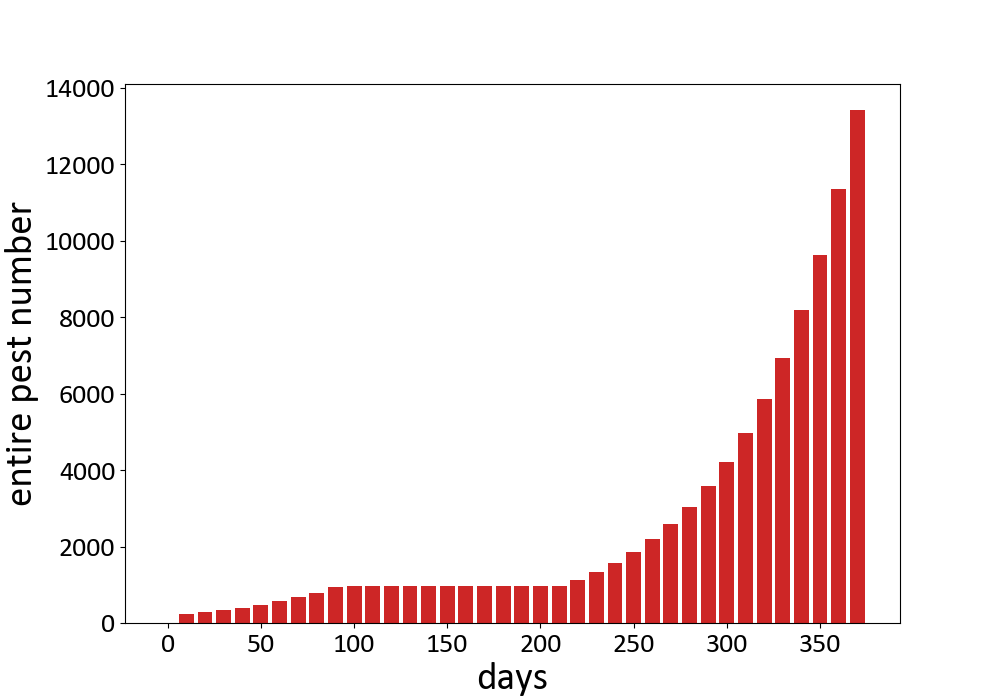
\includegraphics[width=2.5in]{Chapter-2021C/images-2021C/1-sum.png}
    \caption{The entire pest number.}
    \label{fig:2021C-The entire pest number.}
\end{minipage}
\begin{minipage}[t]{0.5\linewidth} 
\centering 
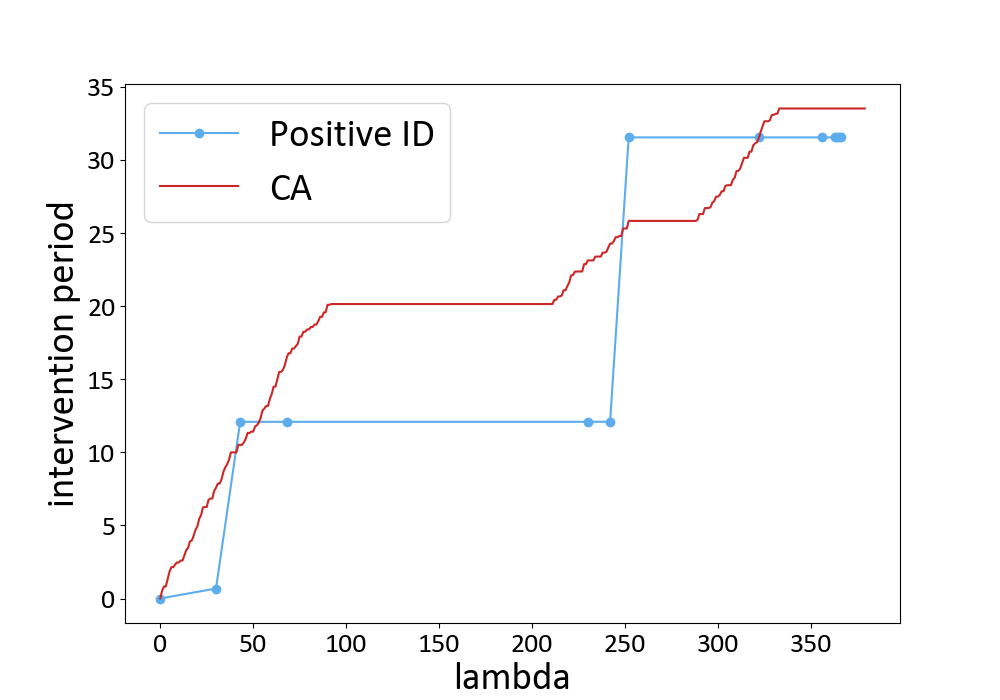
\includegraphics[width=2.5in]{Chapter-2021C/images-2021C/1-distance.png}
    \caption{The longest spread distance.}
    \label{fig:2021C-The longest spread distance.}
\end{minipage} 
\end{figure}

Moreover, we calculate the longest spread distance at each time $t$, convert the cell number to the distance in kilometer, and picture it in Figure \ref{fig:2021C-The longest spread distance.}. In this figure, we compare the longest spread distance of CA simulation with the one of positive reports. We notice that the longest spread distance of  CA simulation is always bigger than the other, which means the simulation have rationality in the reality. The spread can reach at most 34 km after the simulation of 380 days and remains to be a huge potential threat.

\subsection{Precision Analysis}
To do further test towards our simulation, we try to analyze the precision of our model. We incline to point out the place of the positive reports on the picture of the simulation until that day. We extract totally 12 positive reports except for the starting point and the ignored one. We select two of the 12 tests and propose it as followed in Figure \ref{fig:2021C-Positive reports on 2019/10/30.} and Figure \ref{fig:2021C-Positive reports on 2019/12/8.}, where the yellow area denotes our simulation area and the red triangle represents the place of the positive report on that day.

%%插图 标点精确度分析
\begin{figure}[H] 
\begin{minipage}[t]{0.5\linewidth} 
\centering 
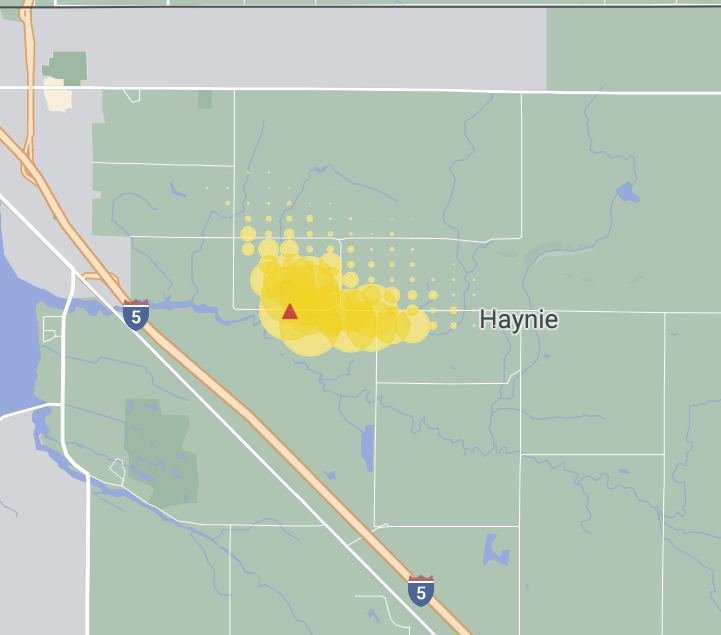
\includegraphics[width=2.2in]{Chapter-2021C/images-2021C/1-10-30.png} 
\caption{Positive reports on 2019/10/30.} 
\label{fig:2021C-Positive reports on 2019/10/30.} 
\end{minipage}
\begin{minipage}[t]{0.5\linewidth} 
\centering 
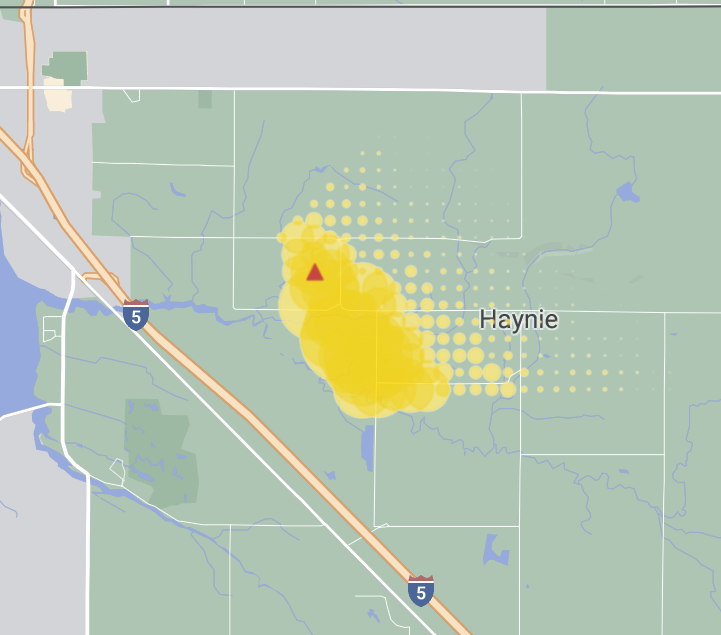
\includegraphics[width=2.2in]{Chapter-2021C/images-2021C/1-12-8.png} 
\caption{Positive reports on 2019/12/8.} 
\label{fig:2021C-Positive reports on 2019/12/8.} 
\end{minipage} 
\end{figure}

Considering all the 12 pictures, we can conclude that the positive reports are all located at the places with high current volumes in the simulation. In our model, we divide the longitude and the latitude into about 1500 and 1000 pieces, respectively. After transformation to meters, one piece of small rectangle represents 150m and 160m of width and length in the real life. So we can say confidently that our model achieves the precision of a $150m \times 150m$ area.

\vspace{1cm}